\documentclass{article}

\usepackage{tikz}
\usepackage{array}
\usepackage{nicefrac}
\usepackage{fullpage}
\usepackage[T1]{fontenc}
\usepackage[sfmath]{kpfonts}
\usepackage[default]{gillius}
\usepackage[normalem]{ulem}

\usetikzlibrary{positioning}
\usetikzlibrary{arrows}
\usetikzlibrary{calc}

\begin{document}
\immediate\write18{./kernel-expt-extra.R}

\pagestyle{empty}

\newcommand{\boxw}{7cm}
\newcommand{\boxh}{2cm}

\begin{tikzpicture}
  \tikzstyle{box}=[minimum width=\boxw, minimum height=\boxh, draw]
  \tikzstyle{next}=[->, >=stealth, thick]

  \node (rect1) [box] { };
  \node at (rect1.north) [anchor=north] {\uline{3 parameter values}};
  \node (b) [above=0.5cm of rect1.south, blue] {\LARGE $\theta_1$};
  \node (r) [left=1.5cm of b, red] {\LARGE $\theta_2$};
  \node (g) [right=1.5cm of b, green] {\LARGE $\theta_3$};

  \node (rect2) [below=of rect1, box] { };
  \node at (rect2.north) [anchor=north] {\uline{300 networks}};
  \node (b) [above=4pt of rect2.south] {
    \begin{tabular}{m{0.5cm} m{1cm} m{0.5cm} m{1cm} m{0.5cm} m{1cm}}
      
\includegraphics[width=1cm]{tinynet1} & $\times$ 100 &
      
\includegraphics[width=1cm]{tinynet2} & $\times$ 100 &
      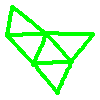
\includegraphics[width=1cm]{tinynet3} & $\times$ 100
    \end{tabular}
  };

  \node (rect3) [below=of rect2, box] { };
  \node at (rect3.north) [anchor=north] {\uline{300 epidemics}};
  \node (b) [above=4pt of rect3.south] {
    \begin{tabular}{m{0.5cm} m{1cm} m{0.5cm} m{1cm} m{0.5cm} m{1cm}}
      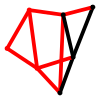
\includegraphics[width=1cm]{tinyepi1} & $\times$ 100 &
      
\includegraphics[width=1cm]{tinyepi2} & $\times$ 100 &
      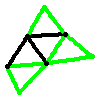
\includegraphics[width=1cm]{tinyepi3} & $\times$ 100
    \end{tabular}
  };

  \node (rect4) [below=of rect3, box] { };
  \node at (rect4.north) [anchor=north] {\uline{300 transmission trees}};
  \node (b) [above=4pt of rect4.south] {
    \begin{tabular}{m{0.5cm} m{1cm} m{0.5cm} m{1cm} m{0.5cm} m{1cm}}
      
\includegraphics[width=1cm]{tinytree1} & $\times$ 100 &
      
\includegraphics[width=1cm]{tinytree2} & $\times$ 100 &
      
\includegraphics[width=1cm]{tinytree3} & $\times$ 100
    \end{tabular}
  };

  \node (rect5) [right=of rect1, box] { };
  \node at (rect5.north) [anchor=north, text width=\boxw, align=center] {
    \uline{42 kernel matrices ($300 \times 300$)} \\ \vspace{4pt}
    $\lambda$ = \{ \nicefrac18, \nicefrac14, \nicefrac12, 1, 2, 4, 8 \} \\
    $\sigma$ = \{ 0.2, 0.3, 0.4 \} \\
    nLTT = \{ yes, no \} \\
  };

  \node (rect6) [below=of rect5, box] { };
  \node at (rect6.north) [anchor=north, text width=\boxw, align=center] {
    \uline{42 cross validations} \\ \hfill \\
    R$^2$ $\times$ 42
  };

  \node (rect7) [below=of rect6, box] { };
  \node at (rect7.north) [anchor=north, text width=\boxw, align=center] {
    \uline{optimal kernel meta-parameters} \\ \hfill \\
    $\lambda$ = 4,\; $\sigma$ = 0.3,\; nLTT = no
  };

  \node (rect8) [below=of rect7, minimum width=\boxw, minimum height=\boxh,
                 align=center, text width=\boxw] {
    repeat 8 times \\
    \vspace{4pt}
    infected nodes = \{ 500, 1000, 2000 \} \\
    sampled nodes = \{ 100, 500, 1000 \}
  };

  \coordinate [left=0.5 of rect5.west] (r5w);
  \coordinate [below=0.5cm of r] (r1ssw);
  \coordinate [below=of r1ssw] (r2nnw);
  \coordinate [below=0.5cm of g] (r1sse);
  \coordinate [below=of r1sse] (r2nne);
  \coordinate [below=3.5cm of r] (r2ssw);
  \coordinate [below=3.5cm of g] (r2sse);
  \coordinate [below=4.5cm of r] (r3nnw);
  \coordinate [below=4.5cm of g] (r3nne);
  \coordinate [below=6.5cm of r] (r3ssw);
  \coordinate [below=6.5cm of g] (r3sse);
  \coordinate [below=7.5cm of r] (r4nnw);
  \coordinate [below=7.5cm of g] (r4nne);
  \coordinate [below=0.5cm of rect4.north east] (r4ene);
  \coordinate [above=0.5cm of rect4.south east] (r4ese);

  \draw[next] (r1ssw) -- (r2nnw);
  \draw[next] (r1ssw) -- ($(r2nnw) + (-0.5cm, 0cm)$);
  \draw[next] (r1ssw) -- ($(r2nnw) + (0.5cm, 0cm)$);
  \draw[next] (r1sse) -- (r2nne);
  \draw[next] (r1sse) -- ($(r2nne) + (-0.5cm, 0cm)$);
  \draw[next] (r1sse) -- ($(r2nne) + (0.5cm, 0cm)$);
  \draw[next] (rect1.south) -- (rect2.north);
  \draw[next] (rect1.south) -- ($(rect2.north) + (-0.5cm, 0cm)$);
  \draw[next] (rect1.south) -- ($(rect2.north) + (0.5cm, 0cm)$);
  \draw [next] (rect2) -- (rect3);
  \draw [next] (r2ssw) -- (r3nnw);
  \draw [next] (r2sse) -- (r3nne);
  \draw [next] (rect3) -- (rect4);
  \draw [next] (r3ssw) -- (r4nnw);
  \draw [next] (r3sse) -- (r4nne);
  \draw [next] (rect4.east) -| (r5w) -- (rect5);
  \draw [thick] (r4ene) -- ++ (0.5cm, -0.5cm);
  \draw [thick] (r4ese) -- ++ (0.5cm, 0.5cm);
  \draw [next] (rect5) -- (rect6);
  \draw [next] (rect6) -- (rect7);
\end{tikzpicture}

\end{document}
